\documentclass[journal]{IEEEtran}

\usepackage{graphicx}
\usepackage{amsmath}
\usepackage{array, tabularx}


\title{Operational Amplifiers: Behaviors \& Implementation}
\author{Aidan Sharpe \& Elise Heim}

\begin{document}
\maketitle

\begin{abstract}
    In this lab, several behaviors and topologies of operational amplifiers were tested. Behaviors analyzed include isolation, positive \& negative feedback, and comparison. Topologies used include the unity gain follower, the non-inverting amplifier, the astable multivibrator, and the differential amplifier. 
\end{abstract}

\section{Background} 
\IEEEPARstart{A}{mplifiers} can be found almost everywhere. In just your day-to-day life you will use them in your phone, in your car, and in undersea communications cables. They are a critical technology globally, necessary for many products in the modern world.

Amplifiers perform a simple task: boosting (\textit{amplifying}) a signal. There are several varieties of amplifiers, but for many purposes, the common operational amplifier is used.

\section{Introduction}
Operational amplifiers, commonly referred to as simply "op-amps" are a type of amplifier with several key properties: isolation, comparison, and amplifier gain. By applying these properties, several rather nifty behaviors emerge.

The following is an overview of several applications and behaviors of op-amps as observed in a laboratory setting.

\section{Slew Rate}
The slew rate of an op-amp is the rate at which it can switch from one voltage to another. As seen in \textit{Fig. \ref{fig:osc_slew_rate}}, voltage does not instantaneously switch, rather it climbs at a steady rate from one point to another. By analyzing the rate of change of voltage with respect to time, the slew rate of any op-amp can be calculated.

\begin{figure}[h]
    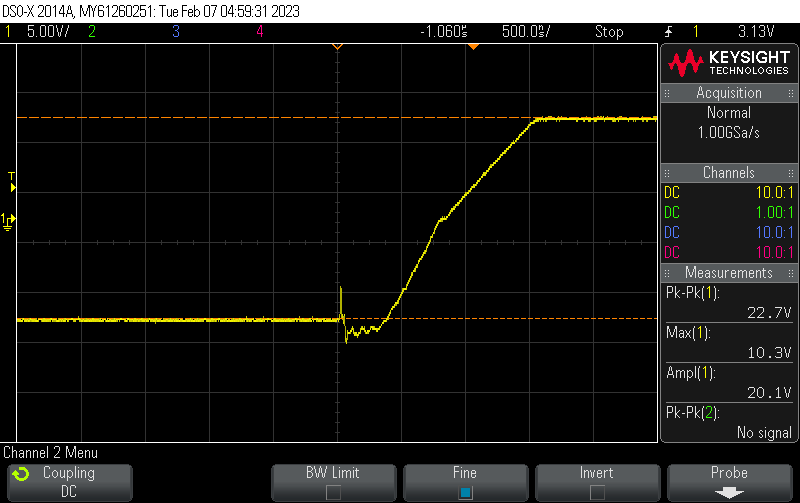
\includegraphics[scale=0.3]{Media/slew_rate.png}
    \caption[short]{Analyzing Slew Rate}
    \label{fig:osc_slew_rate}
\end{figure}

\section{The Unity Gain Follower}
The unity gain follower is the topology that extracts the pure essence of the isolation property of an op-amp---they can emulate input behavior at the output without affecting the input. They are extremely useful when input electronics are sensitive or their properties must be protected.

As seen in \textit{Fig. \ref{fig:sch_unity_gain}}, the output signal is identical to the input signal. However, they are not connected. The op-amp is driving the output signal with a separate power supply and mimicking the signal coming in.

\begin{figure}[h]
    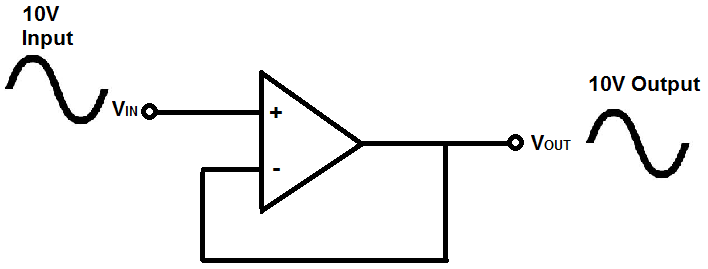
\includegraphics[scale=0.45]{Media/Voltage-follower-example.png}
    \caption[short]{Unity Gain Follower Schematic}
    \label{fig:sch_unity_gain}
\end{figure}

\section{Controlling the Gain}
The amplifier gain, $A$ of an operational amplifier is an arbitrary, often quite high, value that is determined through the manufacturing process. It is very difficult to control during production, but as long as it is a reasonably high value, the exact number becomes irrelevant during application.

Looking at \textit{Eqn. \ref{eqn:op_amp_out}}, the amplifier gain, $A$, plays a role in the output. However, this only occurs when there is no feedback. 

\begin{equation}
    V_{out} = A(V_P - V_N)
    \label{eqn:op_amp_out}
\end{equation}

When there \textit{is} feedback, the amplifier gain plays a negligible role in $V_{out}$, given that $A$ is a sufficiently high value. This is because in a circuit with negative feedback, the amount the output voltage is affected by the amplifier gain is an inverse proportion. A simple inverting amplifier, shown in \textit{Fig. \ref{fig:sch_inverting_amp}} has an output voltage determined through \textit{Eqn. \ref{eqn:inverting_amp_out}}.

\begin{figure}[h]
    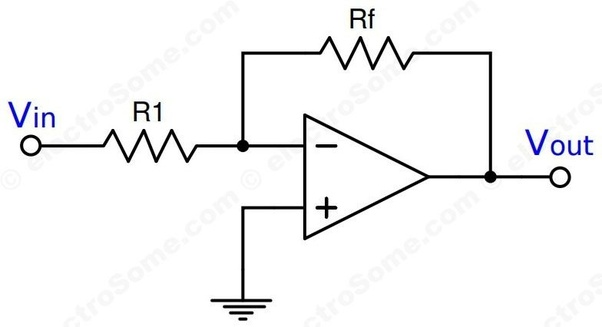
\includegraphics[scale=0.4]{Media/main-qimg-ff6c97a856f809327a49099f4cc0167e.jpeg}
    \caption[short]{Inverting Amplifier Schematic}
    \label{fig:sch_inverting_amp}
\end{figure}

\begin{equation}
    V_{out} = -V_{in}\left(\frac{R_f}{R_1}\right)
    \label{eqn:inverting_amp_out}
\end{equation}

\begin{equation}
    V_{out} = V_{in}\left(1 + \frac{R_f}{R_1}\right)
    \label{eqn:non-inverting_amp_out}
\end{equation}

In comparing \textit{Eqn. \ref{eqn:inverting_amp_out}} and \textit{Eqn. \ref{eqn:non-inverting_amp_out}} it becomes obvious that each setup has its pros and cons. In both cases, gain is affected only by the values of $R_1$ and $R_f$, so it can be fine-tuned to a specific value. However, while the math is a little simpler of the inverting case, the output is, well, inverted. On the other hand, the math for the non-inverting case is ever-so-slightly more complex, but the signal has the same polarity.

For example, one task was to construct an amplifier with a gain of positive ten. Again referencing \textit{Eqn. \ref{eqn:non-inverting_amp_out}} the ratio of $R_f:R_1$ must be 9 since the gain is one greater than the ratio. If the task had rather been to build an amplifier with a gain of negative ten, calculating a $1:10$ ratio of resistor values would have been a little easier.

After constructing the non-inverting amplifier, as seen in \textit{Fig. \ref{fig:osc_non-inverting}}, the signal was spot on.

\begin{figure}[h]
    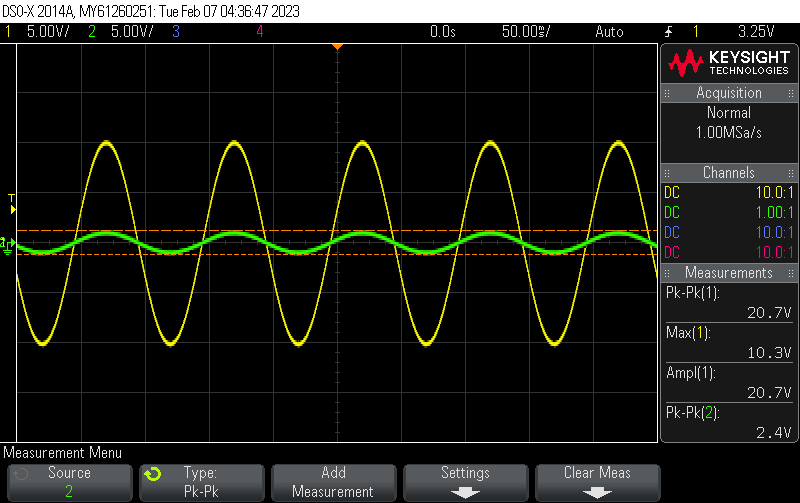
\includegraphics[scale=0.3]{Media/wiggle_10x.png}
    \caption[short]{Analyzing Non-inverting Amplifier Output}
    \label{fig:osc_non-inverting}
\end{figure}

\section{The Astable Multivibrator}
The astable multivibrator is a really helpful circuit. It uses a combination of the comparison property of the op-amp and the transient response property of a capacitor to create an oscillating square wave. Its schematic and output behavior are seen in \textit{Fig. \ref{fig:sch_multivibrator}}.

\begin{figure}[h]
    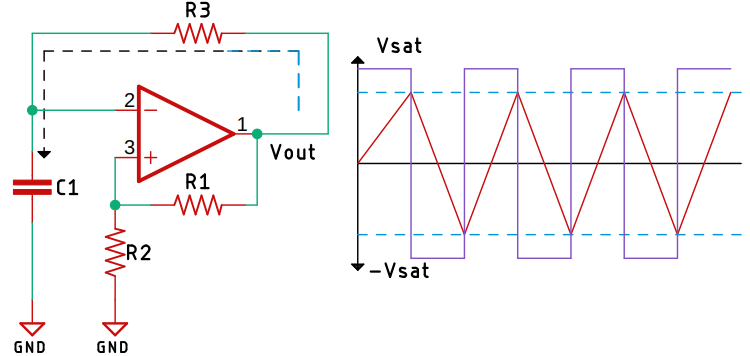
\includegraphics[scale=0.3]{Media/Op-amp-Astable-Multivibrator-Working.png}
    \caption[short]{Astable Multivibrator Schematic and Output}
    \label{fig:sch_multivibrator}
\end{figure}

\begin{equation}
    T = 2R_3C \times \ln\left({\frac{1+\beta}{1-\beta}}\right)
    \label{eqn:astable_period}
\end{equation}
\\
Where:
\begin{tabularx}{\linewidth}{>{$}r<{$} @{${}={}$} X}
    \beta & $\frac{R_2}{R_1 + R_2}$;\\
    T & Period of oscillation\\
\end{tabularx}
\\
\\

Given \textit{Eqn. \ref{eqn:astable_period}}, choosing a value, $\beta$, such that $\frac{1+\beta}{1-\beta} \approx  e$ will make it possible to tune the period of oscillation using $R_3$ alone. To achieve this, $R_2$ should be about $86\%$ of the resistance of $R_1$.

Lab resistors have an uncertainty of $\pm5\%$. Using a $39 K\Omega$ resistor for $R_1$ and a $33 K\Omega$ resistor for $R_2$ will give us a $\beta$ of approximately $e$. 

\begin{figure}[h]
    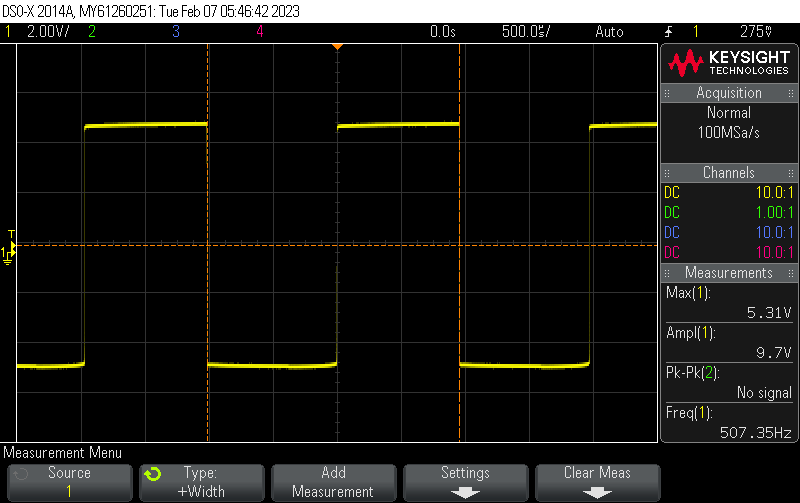
\includegraphics[scale=0.3]{Media/astable_500hz.png}
    \caption[short]{Analyzing Astable Multivibrator Output}
    \label{fig:osc_multivibrator}
\end{figure}

\section{Conclusion}
It should be clear that the unique properties of operational amplifiers have a diverse set of applications. The ability to isolate each side of the amplifier means that the behaviors on either side do not affect each other. The comparison behavior allows for fine-tuning output gain and creating an oscillating output from a direct current source. These are just a few isolated (no pun intended) use cases for op-amps, and their behaviors can be extended into many useful applications.
\end{document}